\chapter{Multi class classification}

\section{Introduzione}

	\subsection{Classificazione binaria}
	Si \`e definita la classificazione binaria come la task in cui dati:
	\begin{itemize}
		\item Uno spazio di input $\mathcal{X}$.
		\item Una distribuzione sconosciuta $\mathcal{D}$ su $\mathcal{X}\times\{-1,+1\}$.
		\item Un training set $D$ campionato da $\mathcal{D}$
	\end{itemize}
	Si deve computare una funzione $f$ che minimizza $\mathbb{E}_{(x,y)\sim\mathcal{D}}[f(x)\neq y]$
	
	\subsection{Classificazione multi classe}
	La classificazione multiclasse \`e l'estensione naturale della classificazione binaria.
	L'obiettivo \`e quello di assegnare una label discreta a degli esempi.
	La differenza \`e che ora ci sono $k>2$ classi da cui scegliere.
	Dati pertanto:
	\begin{itemize}
		\item Uno spazio di input $\mathcal{X}$ e un numero di classi $K$.
		\item Una distribuzione sconosciuta di $\mathcal{D}$ su $\mathcal{X}\times[K]$.
		\item Un training set $D$ campionato da $\mathcal{D}$.
	\end{itemize}
	Si deve computare una funzione $f$ che minimizza $\mathbb{E}_{(x,y)\sim\mathcal{D}}[f(x)\neq y]$.
	
		\subsubsection{K nearest neighbours}
		Si noti come una \emph{K-NN} per classificare un esempio $d$ trova i $k$ vicini di $d$ e sceglie la label in presenza maggiore tra i $k$ vicini pi\`u prossimi.
		Non necessita pertanto di cambi algoritmici nel caso della multi class classification.
		
		\subsubsection{Decision tree}
		I decision tree non richiedono cambi algoritmici per la multi class classification.
	
	\subsection{Approccio black box alla multi class classification}
	Dato un classificatore binario questo si pu\`o usare per risolvere il problema della multiclass classification.
	Si noti come un perceptron oltre al risultato pu\`o anche dare un punteggio di confidenza.
	Inoltre siccome una linea non \`e sufficiente per dividere le classi se ne possono usare diverse.

\section{One versus all \emph{OVA}}
Nell'approccio \emph{OVA} nel training si definisce per ogni label $L$ un problema binario in cui:
\begin{itemize}
	\item Tutti gli esempi con la label $L$ sono positivi.
	\item Tutti gli altri esempi sono negativi.
\end{itemize}


\begin{figure}
	\centering
	\begin{minipage}{.5\textwidth}
		\centering
		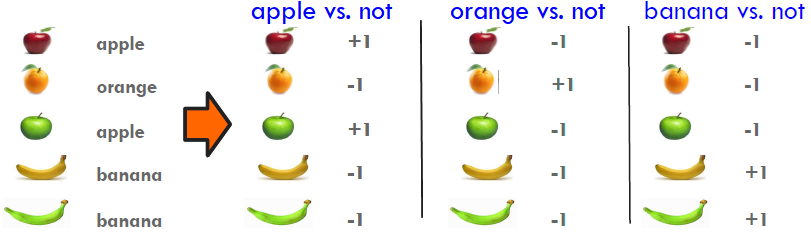
\includegraphics[width=1\linewidth]{imgs/chapter6/img0}
		\caption{Esempio OVA}
		\label{fig:chapter06-00}
	\end{minipage}%
	\begin{minipage}{.5\textwidth}
		\centering
		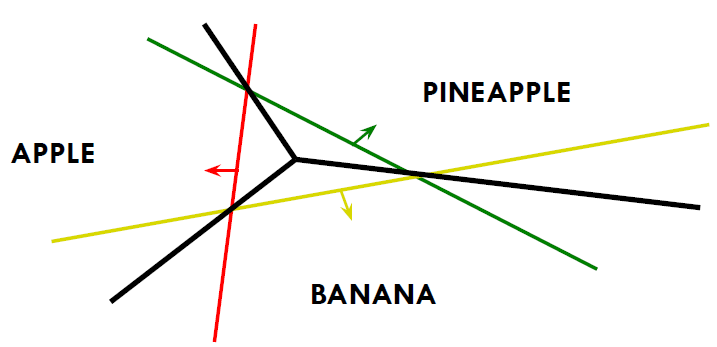
\includegraphics[width=0.8\linewidth]{imgs/chapter6/img1}
		\caption{Esempio OVA. Le frecce indicano il lato positivo della linea}
		\label{fig:chapter06-01}
	\end{minipage}
\end{figure}

In pratica si imparano $L$ diversi modelli di classificazione.
Si ricordi come il classificatore divide il piano in due semipiani.

	\subsection{Ambiguit\`a}
	In questo caso si formano pertanto delle zone in cui si creano delle ambiguit\`a. 
	Nella figura \ref{fig:chapter06-01} \`e possibile che un esempio si trovi nel lato positivo di due linee contemporaneamente.
	Se il classificatore non fornisce confidence e c'\`e ambiguit\`a si sceglie una delle label in conflitto.
	Nella maggior parte dei casi i classificatori forniscono confidence, allora in questo caso si:
	\begin{itemize}
		\item Si sceglie il positivo con confidence maggiore.
		\item Se nessuno \`e positivo si sceglie il negativo con confidence minore.
	\end{itemize}
	La confidence nel perceptron si calcola come distanza dall'iperpiano stabilito dalla prediction.
	
	\subsection{Algoritmi}
	
\begin{algorithm}
\DontPrintSemicolon
\SetKwComment{comment}{$\%$}{}
\SetKw{Int}{int}
\SetKw{To}{to}
\SetKw{IsNot}{is not}
\SetKw{Not}{not}
\SetKw{Return}{Return}
\SetKwData{Item}{item}
\SetKwFunction{BinaryTrain}{BinaryTrain}
\SetKwFunction{Ova}{OneVersusAllTrain}

\caption{\protect\Ova{$D^{multiclass}$, \protect\BinaryTrain{}}}

\For{$i\ =\ 1$ \To $K$}{
	$D^{bin}$ = relabel $D^{multiclass}$ in modo che $i$ \`e positivo e $\neq i$ \`e negativo\;
	$f_i$ = \BinaryTrain{$D^{bin}$}\;
}
\Return $f_1,\dots, f_K$

\end{algorithm}

	
	Con $k$ categorie si avranno $k$ modelli.
	
	\begin{algorithm}[H]
\DontPrintSemicolon
\SetKwComment{comment}{$\%$}{}
\SetKw{Int}{int}
\SetKw{To}{to}
\SetKw{IsNot}{is not}
\SetKw{Not}{not}
\SetKw{Return}{Return}
\SetKwData{Item}{item}
\SetKwFunction{BinaryTrain}{BinaryTrain}
\SetKwFunction{Ova}{OneVersusAllTest}
\SetKwFunction{Max}{max}

\caption{\protect\Ova{$f_1,\dots,f_K$, $\hat{x}$}}

score = $\langle 0,\dots, 0\rangle$		\comment{Inizializza $K$ score a $0$}

\For{$i\ =\ 1$ \To $K$}{
	y = $f_i(\hat{x})$\;
	$score_i\ =\ score_i + y$\;
}
\Return \Max{score}\;

\end{algorithm}


\section{All versus all \emph{AVA}}
Un approccio alternativo consiste nel gestire il problema della classificazione multi classe decomponendolo in problemi di classificazione binaria.
Questo approccio viene detto anche all pairs.
Si classificano $\frac{K(K-1)}{2}$ classificatori in modo che
$$F_{ij}, 1\le i< j \le K$$
Sia il classificatore che discrimina la classe $i$ contro la classe $j$.
Questo classificatore riceve tutti gli esempi della classe $i$ come positivi e tutti gli esempi della classe $j$ come negativi.
Quando arriva un punto di test si valuta su tutti i classificatori $F_{ij}$.
Ogni volta che $F_{ij}$ predice positivo la classe $i$ prende un voto, altrimenti lo prende $j$.
Dopo aver eseguito tutti i $\frac{K(K-1)}{2}$ classificatori la classe con pi\`u voti decide la label.

\begin{figure}
	\centering
	\begin{minipage}{.5\textwidth}
		\centering
		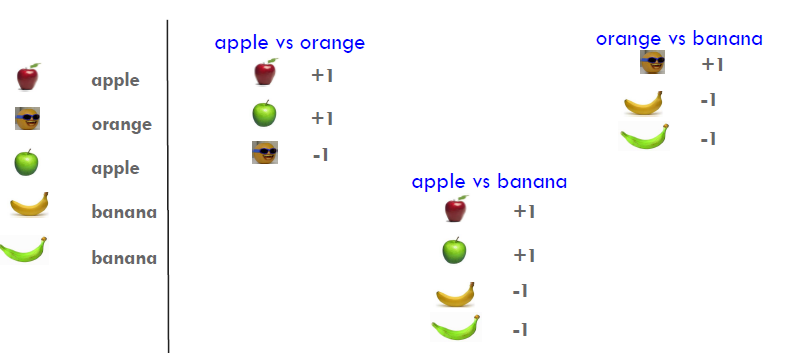
\includegraphics[width=0.8\linewidth]{imgs/chapter6/img2}
		\caption{Esempio \emph{AVA}}
		\label{fig:chapter06-02}
	\end{minipage}%
	\begin{minipage}{.5\textwidth}
		\centering
		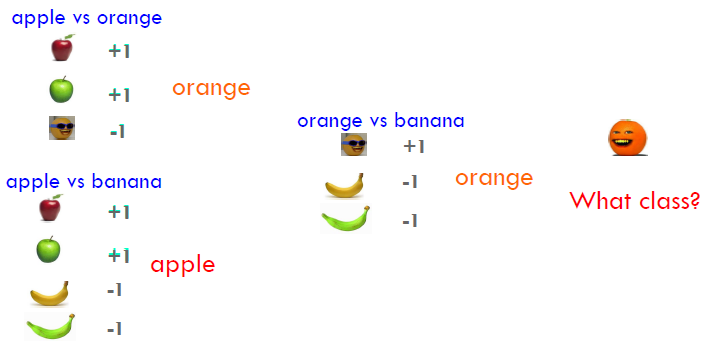
\includegraphics[width=0.8\linewidth]{imgs/chapter6/img3}
		\caption{Esempio \emph{AVA}}
		\label{fig:chapter06-03}
	\end{minipage}
\end{figure}
La maggioranza dice \emph{orange}, dunque assegneremo la label \emph{orange} \ref{fig:chapter06-03}.
	\subsection{\emph{AVA} training}
	Per ogni coppia di label si addestra un classificatore che le distingue:\\
	\begin{algorithm}[H]
\DontPrintSemicolon
\SetKwComment{comment}{$\%$}{}
\SetKw{Int}{int}
\SetKw{To}{to}
\SetKw{IsNot}{is not}
\SetKw{Not}{not}
\SetKw{Return}{Return}
\SetKwData{Item}{item}
\SetKwFunction{BinaryTrain}{BinaryTrain}
\SetKwFunction{Ava}{AllVersusAllTrain}
\SetKwFunction{Max}{max}

\caption{\protect\Ava{}}
\For{i = 1 \To number of labels}{
	\For{j = i + 1 \To number of labels}{
		train a classifier $F_{ij}$ to distinguish between $label_j$ and $label_i$\;
		create a dataset with all examples with $label_j$ labeled positive and with $label_i$ negative\;
		Train classifier $F_{ij}$ su questo sottoinsieme di dati\;
	}
}
\end{algorithm}




	\subsection{\emph{AVA} classification}
	Per classificare un esempio $x$ lo si classifica per ogni classificatore $F_{ij}$.
	Per scegliere la classe finale si pu\`o:
	\begin{itemize}
		\item Considerare la maggioranza.
		\item Considerare un voto pesato basato sulla confidence:
		\begin{itemize}
			\item $y = F_{ij}(x)$.
			\item $score_j +=y$.
			\item $score_i -=y$.
		\end{itemize}
		Lo score viene cambiato in quanto se $y$ \`e positivo il classificatore lo pensa di tipo $j$, se negativo lo pensa di tipo $i$ e pertanto lo score viene aggiornato di conseguenza.
	\end{itemize}
	
	\subsection{Algoritmi}
	\begin{algorithm}
\DontPrintSemicolon
\SetKwComment{comment}{$\%$}{}
\SetKw{Int}{int}
\SetKw{To}{to}
\SetKw{IsNot}{is not}
\SetKw{Not}{not}
\SetKw{Return}{Return}
\SetKwData{Item}{item}
\SetKwFunction{BinaryTrain}{BinaryTrain}
\SetKwFunction{Ava}{AneVersusAllTrain}

\caption{\protect\Ava{$D^{multiclass}$, \protect\BinaryTrain{}}}
$f_{ij}\ =\ \emptyset,\ \forall 1\le i < j \le K$\;
\For{$i\ =\ 1$ \To $K\ -\ 1$}{
	$D^{pos}\ =\ $ all $x\in D^{multiclass}$ labeled $i$\;
	\For{$j\ =\ j\ +\ 1$ \To $K$}{
		$D^{neg}\ =$ all $x\in D^{multiclass}$ labeled $j$\;
		$D^{bin}\ =\ \{(x, +1):x\in D^{pos}\}\cup\{(x,-1):x\in D^{neg}\}$\;
		$f_{ij}$ = \BinaryTrain{$D^{bin}$}\;
	}
}

\Return all $f_{ij}$

\end{algorithm}

	\begin{algorithm}[H]
\DontPrintSemicolon
\SetKwComment{comment}{$\%$}{}
\SetKw{Int}{int}
\SetKw{To}{to}
\SetKw{IsNot}{is not}
\SetKw{Not}{not}
\SetKw{Return}{Return}
\SetKwData{Item}{item}
\SetKwFunction{BinaryTrain}{BinaryTrain}
\SetKwFunction{Ava}{AllVersusAllTest}
\SetKwFunction{Max}{max}

\caption{\protect\Ava{all $f_{ij}$, $\hat{x}$}}

score = $\langle 0,\dots, 0\rangle$		\comment{Inizializza $K$ score a $0$}

\For{$i\ =\ 1$ \To $K\ -\ 1$}{
	\For{$j\ =\ i\ +\ 1$ \To $K$}{
		y = $f_{ij}(\hat{x})$\;
		$score_i\ =\ score_i + y$\;
		$score_j\ =\ score_j - y$\;
	}
}
\Return \Max{score}\;

\end{algorithm}

	
	\section{Confronto tra \emph{OVA} e \emph{AVA}}
	
	\subsection{Tempo di training}
	\emph{AVA} impara pi\`u classificatori ma il training set \`e molto pi\`u piccolo pertanto tende ad essere pi\`u veloce se le label sono equamente bilanciate.
	
	\subsection{Tempo di test}
	Avendo \emph{AVA} pi\`u classificatori \`e tipicamente pi\`u lenta.
	
	\subsection{Errori}
	\emph{AVA} fa training con data sets pi\`u bilanciati, ma avendo pi\`u classificatori i test tendono ad avere pi\`u possiblit\`a di errori.

\section{Riassunto}
Se vengono usati classificatori binari viene tipicamente utilizzata  \emph{OVA}, altrimenti si usa un classificatore che permette label multiple come \emph{DT} o \emph{K-NN}, nonostante altri metodi pi\`u sofisticati siano meglio.

\section{Multiclass evaluation}
Per computare l'accuratezza nella predizione di una classe $c$ si pu\`o usare la misura di predizione $Pr=\frac{TP}{TP+FP}$ dove $TP$ sono le predizioni corrette e $FP$ le predizioni scorrette \ref{fig:chapter06-04}.

	\subsection{Microaveraging}
	Nel microaveraging si fa la media sugli esempi.
	Considerando $n$ classi si calcola come:
	$$Pr=\dfrac{\sum\limits_{i=1}^nTP_{c_i}}{\sum\limits_{i=1}^n(TP_{c_i}+FP_{c_i})}$$
	
	\subsection{Macroaveraging}
	Nel macroaveraging si calcola lo score di valutazione o accuratezza per ogni label e poi si fa la media tra le label.
	Questo in quanto d\`a pi\`u enfasi a label pi\`u rare e permette un'altra dimensione di analisi.
	$$Pr=\dfrac{\sum\limits_{c\in C}Pr_c}{|C|}$$
	
	\begin{figure}
		\centering
		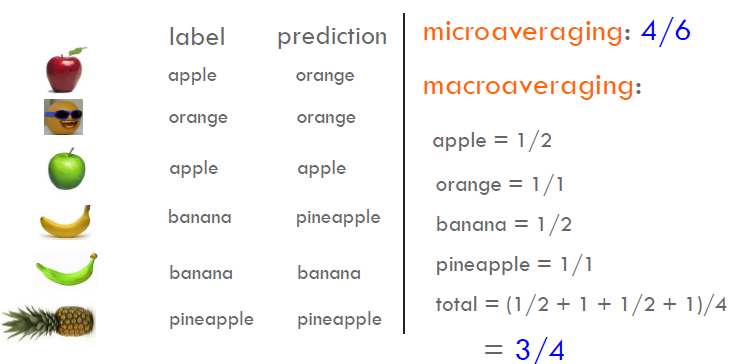
\includegraphics[width=0.6\linewidth]{imgs/chapter6/img4}
		\caption{Multiclass evaluation}
		\label{fig:chapter06-04}
	\end{figure}
	
	\subsection{Confusion matrix}
	La confusion matrix \`e una matrice in cui $(i, j)$ rappresenta il numero di esempi con label $i$ predetti avere label $j$.
	Viene spesso espressa come percentuale.
	Nel caso di una classificazione a $k$ classi sar\`a di dimensione $k\times k$.
	La performance \`e buona nel caso in cui la diagonale presenti le percentuali pi\`u alte.
